\documentclass[10pt, twoside]{report}

\usepackage[T1]{fontenc}
\usepackage[utf8]{inputenc}
%%\usepackage[us]{babel}
\usepackage{helvet}
\usepackage[a4paper,width=180mm,top=25mm,bottom=25mm,bindingoffset=6mm]{geometry}
\usepackage[framemethod=default]{mdframed}
\usepackage{lipsum,titlesec,xcolor,fancyhdr,array,multicol,float,graphicx,wrapfig,subcaption}
\usepackage{fontspec,todonotes,enumitem,comment,capt-of,amsmath,booktabs}
\usepackage[colorlinks]{hyperref}
\usepackage[font=scriptsize]{caption}
\usepackage[sorting=none]{biblatex}
\addbibresource{references.bib}

\DeclareCaptionLabelFormat{andtable}{#1˜#2 \& \tablename˜\thetable}

\renewcommand{\familydefault}{\sfdefault}

\graphicspath{{images/}}

%% define size for chapter initial page:
\usepackage{titlesec, blindtext, color}
\definecolor{gray75}{gray}{0.75}
\newcommand{\hsp}{\hspace{20pt}}
\titleformat{\chapter}[hang]{\Huge\bfseries}{\thechapter\hsp\textcolor{gray75}{|}\hsp}{0pt}{\Huge\bfseries}

\titlespacing*{\chapter}{0pt}{-60pt}{20pt} %% change spacing
%%%%%%%%%%

\floatstyle{plain}
\restylefloat{figure}

\pagestyle{fancy}
\fancyhf{}
\renewcommand{\chaptermark}[1]{ \markboth{#1}{} }
\renewcommand{\sectionmark}[1]{ \markright{#1}{} }
\fancyhead[LE]{\itshape{ \fontsize{10}{12} \selectfont \leftmark}}
\fancyhead[RE, LO]{\thepage}
\fancyhead[RO]{\itshape{\fontsize{10}{12} \selectfont \rightmark}}
\renewcommand\headrulewidth{0pt}

 \hypersetup{
     colorlinks,
     citecolor= green,
     filecolor=black,
     linkcolor= black,
     urlcolor=blue
 }


\begin{document}
    \begin{titlepage}
    \centering
    
\includegraphics[width=0.30\textwidth]{images/cherubino_black.pdf}\par\vspace{1cm}
    {\scshape\LARGE Università di Pisa \par}
    \vspace{1cm}
    {\scshape\ Social Network Analysis \\A.A. 2017/2018\par}
    \vspace{1.5cm}
    {\huge\bfseries Cambridge Analytica and Facebook: \\ The Scandal and the Fallout on Twitter\\ \par}
    \vspace{2cm}
    {\Large Gianmarco Ricciarelli 555396 \\ Stefano Carpita 304902 \par}
    \vfill

\begin{flushright}    
  \textit{Data drives all we do.}\\
\vspace{2 mm}
Cambridge Analytica main slogan.
\end{flushright}

\vspace{4 mm}
    
\begin{flushright}    
  \textit{Rules don’t matter for them. \\ For them, this is a war, and it’s all fair.}\\
\vspace{2 mm}
  Christopher Wylie, \\ former datascientist at Cambridge Analytica, about its leaders.
\end{flushright}




  \end{titlepage}


    \pagenumbering{Roman}
    \tableofcontents
    \chapter{The case story}
    \pagenumbering{arabic}

On Saturday 17 of March 2018, the newspapers The Observer and The New York Times broke reports on how the consulting firm Cambridge Analytica harvested private information from the Facebook profiles of more than 50 million users without their permission, making it one of the largest data leaks in the social network’s history. \cite{nyt_17march}. REF OBSERVER

The whistleblower Christopher Wylie, datascientist and former director of research at Cambridge Analytica revealed...
Cambridge Analytica described itself as a company providing consumer research, targeted advertising and other data-related services to both political and corporate clients.

What, Where, Who, Why, Where ?


Timeline da sistemare: \cite{nyt_timeline}
\begin{itemize}

\item March 17, 2018: The Observer and The New York Times publish joint reports on data harvesting by Cambridge Analytica. UK Information Commissioner Elizabeth Denham issues statement that they are “investigating circumstances in which Facebook data may have been illegally acquired and used.” Politicians in US and UK call for investigation.

\item March 19, 2018: Channel 4 News publishes part 1 of their undercover investigation into Cambridge Analytica. Facebook sends investigators to Cambridge Analytica’s offices. UK Information Commissioner orders them to stand down.

\item March 20, 2018: Channel 4 News publishes part 2 of their undercover investigation into Cambridge Analytica, where they boast about getting Donald Trump elected. British MP Damian Collins calls on Facebook to present oral evidence on Cambridge Analytica. Facebook agrees to send former operations manager Sandy Parakilas. Facebook holds internal Q\&A with attorney Paul Grewal to discuss the crisis, but CEO Mark Zuckerberg and COO Sheryl Sandberg do not attend. Cambridge Analytica suspends CEO Alexander Nix. Facebook demands to inspect Christopher Wylie’s phone. FTC opens investigation into Facebook.
\item to be continued...
\end{itemize}

    \chapter{Building the network}

    \begin{figure}[htbp]
      \centering
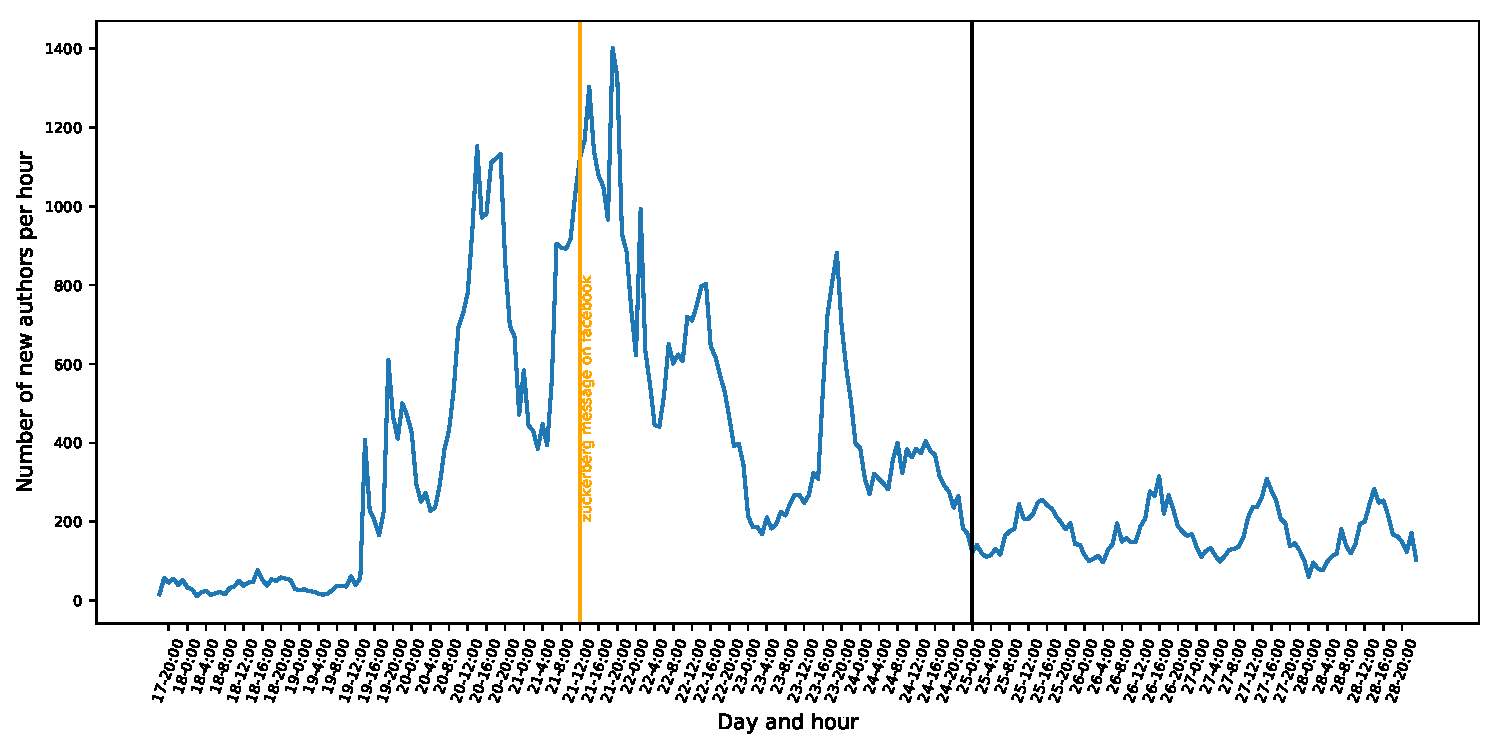
\includegraphics[width=\textwidth]{../../scripts/visualization/imgs/time_history.pdf}
      \caption{New authors time history}
      \label{fig:time_history}
    \end{figure}


    \chapter{Network properties}


    \begin{figure}[htbp]
      \centering
      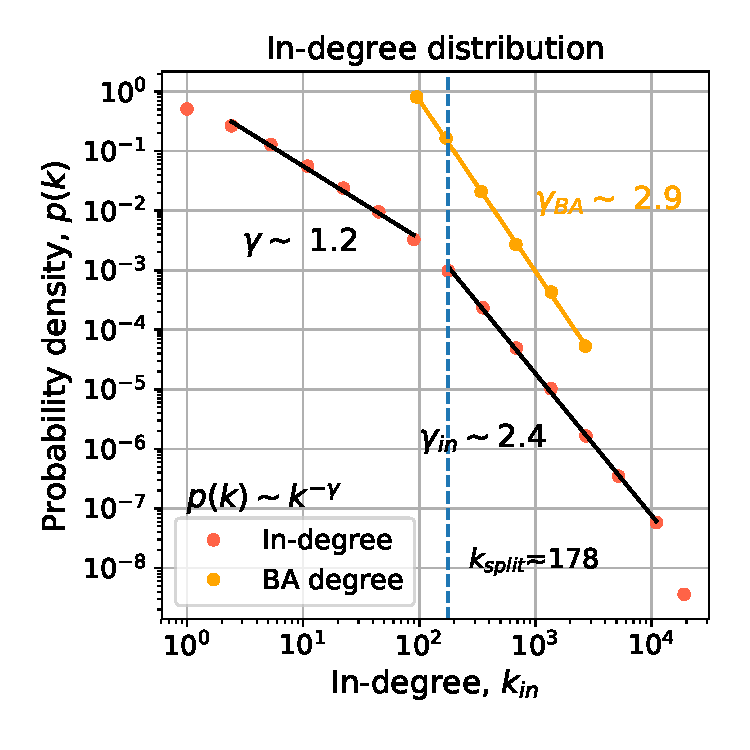
\includegraphics[width=\textwidth]{../../scripts/visualization/imgs/in_degree_distribution.pdf}
      \caption{New authors time history}
      \label{fig:time_history}
    \end{figure}


    \chapter{Network dynamics}

    \chapter{Communities discovery} % (fold)
\label{cha:communities_discovery}

In this chapter we'll provide the results obtained by applying \textbf{K-Clique}, \textbf{Label Propagation},
\textbf{Louvain}, \textbf{Girvan-Newman} and \textbf{Demon} to a sample of $1000$ nodes taken from the original
network. We've chosen to sample the crawled data in order to ease the application of the various algorithms.
Each partition is evaluated by applying an implementation of the scoring functions listed in
\cite{comm_ground_truth}, and, for each algorithm, the results are represented in a table. Together with the
results of the scoring functions are also provided the total number of communities discoverd (Communities), the
number of nodes in the smallest/biggest community (Smallest/Biggest), the hashtags utilized in the biggest
community (Tags) and finally the languages of the users in the biggest community (Langs).

\section{K-Clique} % (fold)
\label{sec:k_clique}
    We have chosen to apply the \textbf{K-Clique} algorithm, described in \cite{k_clique}, to the sample using
    three different values for $k$: $3$, $4$ and $5$, respectively. The results are represented in Table
    \ref{kclique}. As we can see, even if the result is not so good, the best partition is obtained by using $k$
    eguals to $3$, which returns a low modularity partition composed by low degree nodes. It is interesting to
    note that all the biggest partitions returned by the various applications of the algorithm are composed only
    by english speaking users.

    \begin{table}[H]
        \centering
        \begin{subtable}{\textwidth}
            \resizebox{\textwidth}{!}{
                \begin{tabular}{| c | c | c | c | c | c | c | c | c | c |}
                    \hline
                    K & Communities & Biggest & Smallest & Modularity & Conductance & IED & AND &  Tags &
                    Langs \\
                    \hline
                    3 & 29 & 51 & 3 & 0.14 & 0.62 & 0.20 & 2.72 & zuckerberg,
                    cambridgeanalytica, deletefacebook, facebook, facebookgate & English, Deutsch \\
                    \hline
                    4 & 13 & 14 & 4 & 0.020 & 0.68 & 0.21 & 4.23 & cambridgeanalytica, deletefacebook, facebook
                    & English \\
                    \hline
                    5 & 5 & 12 & 5 & 0.011 & 0.63 & 0.23 & 4.83 & cambridgeanalytica, deletefacebook, facebook
                    & English \\
                    \hline
                \end{tabular}
            }
        \end{subtable}
        \caption{Evaluation of the partitions obtained by the application of the K-Clique algorithm.}
        \label{kclique}
    \end{table}

% section k_clique (end)

\section{Label Propagation} % (fold)
\label{sec:label_propagation}
    In Table \ref{labelprop} are represented the results of the application of the \textbf{Label Propagation}
    algorithm, described in \cite{label_propagation}. According to the modularity score the partition provided by
    this algorithm represent a good subdivision of the original network, even if it is composed for the vast
    majority by small communities, as suggested by the high number of communities and the low value for the
    Average Node Degree score. As for the kclique algorithm, it is interesting to note that the biggest community
    is composed only by english speaking users.

    \begin{table}[H]
        \centering
        \begin{subtable}{\textwidth}
            \resizebox{\textwidth}{!}{
                \begin{tabular}{| c | c | c | c | c | c | c | c | c |}
                    \hline
                    Communities & Biggest & Smallest & Modularity & Conductance & IED & AND &  Tags & Langs \\
                    \hline
                    1278 & 136 & 1 & 0.68 & 0.28 & 0.19 & 1.38 & cambridgeanalytica,
                    deletefacebook, privacy, zuckerberg, facebook, facebookgate & Various  \\
                    \hline
                \end{tabular}
            }
        \end{subtable}
        \caption{Evaluation of the partition obtained by the application of the Label Propagaion algorithm.}
        \label{labelprop}
    \end{table}

% section label_propagation (end)

\section{Louvain} % (fold)
\label{sec:louvain}
    The application of the \textbf{Louvain}, described in \cite{louvain}, along with the last iteration of the
    Girvan-Newman algorithm, returns the best partition among all the partitions returned by the other algorithms.
    The results of its application are represented in Table \ref{louvain}. As for the Label Propagation algorithm,
    this partition also is composed by an high number of small communities, composed by nodes with degree betweem
    $1$ and $2$.

    \begin{table}[H]
        \centering
        \begin{subtable}{\textwidth}
            \resizebox{\textwidth}{!}{
                \begin{tabular}{| c | c | c | c | c | c | c | c | c |}
                    \hline
                    Communities & Biggest & Smallest & Modularity & Conductance & IED & AND &  Tags & Langs \\
                    \hline
                    1193 & 133 & 1 & 0.76 & 0.042 & 0.17 & 1.60 & cambridgeanalytica,
                    deletefacebook, privacy, zuckerberg, facebook, facebookgate & Various \\
                    \hline
                \end{tabular}
            }
        \end{subtable}
        \caption{Evaluation of the partition obtained by the application of the Louvain algorithm.}
        \label{louvain}
    \end{table}

% section louvain (end)

\section{Girvan-Newman} % (fold)
\label{sec:girvan_newman}
    For the \textbf{Girvan-Newman} algorithm, described in \cite{girvan_newman}, we've decided to record
    the results of $5$ iterations over the sample network. The results are represented in Table
    \ref{girvan_newman}. As you can see, the first iteration returns a very poor partition, with a low modularity
    score, due to the fact that the edge with the highest betweenness centrality in the starting sample network
    doesn't provide a good grade of separation among the nodes of the network. With the second iteration, and the
    ones after that, there is a consistent improvement either in the modularity score and in the other measures.
    \begin{table}[H]
        \centering
        \begin{subtable}{\textwidth}
            \resizebox{\textwidth}{!}{
                \begin{tabular}{| c | c | c | c | c | c | c | c | c | c |}
                    \hline
                    Iteration & Communities & Biggest & Smallest & Modularity & Conductance & IED & AND &  Tags &
                    Langs \\
                    \hline
                    1 & 1181 & 703 & 1 & 0.17 & 0.00098 & 0.22 & 1.23 & cambridgeanalytica,
                    deletefacebook, privacy, zuckerberg, facebook, facebookgate & Various \\
                    \hline
                    2 & 1182 & 659 & 1 & 0.24 & 0.0019 & 0.21 & 1.27 & cambridgeanalytica,
                    deletefacebook, privacy, zuckerberg, facebook, facebookgate & Various \\
                    \hline
                    3 & 1183 & 588 & 1 & 0.38 & 0.0048 & 0.21 & 1.35 & cambridgeanalytica, deletefacebook, privacy,
                    zuckerberg, facebook, facebookgate & Various \\
                    \hline
                    4 & 1184 & 575 & 1 & 0.40 & 0.0081 & 0.20 & 1.34 & cambridgeanalytica, deletefacebook, privacy,
                    zuckerberg, facebook, facebookgate & Various \\
                    \hline
                    5 & 1185 & 458 & 1 & 0.57 & 0.011 & 0.20 & 1.40 & zuckerberg, cambridgeanalytica, deletefacebook,
                    facebook, facebookgate & Various \\
                    \hline
                \end{tabular}
            }
        \end{subtable}
        \caption{Evaluation of the partition obtained by the application of the Girvan-Newman algorithm.}
        \label{girvan_newman}
    \end{table}

    In general, the partitions returned by the five iterations of the algorithms are all composed by an high number
    of small communities.

% section girvan_newman (end)

\section{Demon} % (fold)
\label{sec:demon}
    Finally in Table \ref{demon} we provide the results of the application of the \textbf{Demon} algorithm,
    described in \cite{demon}, that we tested for three different values of $\epsilon$, $0.25$, $0.50$ and $0.75$,
    respectively. In general, the three partitions are not so good from the point of view of the modularity score,
    with the first application of the algorithm beign the best among the three
    Contrary to the results obtained by the application of the other algorithms, the partitions for the Demon
    algorithm are all composed by a small number of communities, with the last one being the "denser" one, which
    are composed by nodes with a degree between $3$ and $4$.

    \begin{table}[H]
        \centering
        \begin{subtable}{\textwidth}
            \resizebox{\textwidth}{!}{
                \begin{tabular}{| c | c | c | c | c | c | c | c | c | c |}
                \hline
                Epsilon & Communities & Biggest & Smallest & Modularity & Conductance & IED & AND &  Tags & Langs \\
                \hline
                0.10 & 10 & 147 & 4 & 0.07 & 0.46 & 0.082 & 4.41 &
                zuckerberg, cambridgeanalytica, deletefacebook, facebook, facebookgate & Various \\
                \hline
                0.25 & 11 & 63 & 4 & 0.095 & 0.44 & 0.094 & 4.31 &
                zuckerberg, cambridgeanalytica, deletefacebook, facebook, facebookgate & English, Deutsch \\
                \hline
                0.50 & 21 & 43 & 4 & 0.11 & 0.57 & 0.10 & 4.15 &
                zuckerberg, cambridgeanalytica, deletefacebook, facebook, facebookgate & English, Deutsch \\
                \hline
                0.75 & 39 & 25 & 4 & 0.62 & 0.51 & 0.12 & 3.96 &
                zuckerberg, cambridgeanalytica, deletefacebook, facebook, facebookgate & English, Deutsch \\
                \hline
                0.90 & 89 & 24 & 4 & 0.071 & 0.68 & 0.15 & 3.65 &
                zuckerberg, cambridgeanalytica, deletefacebook, facebook, facebookgate & English, Deutsch \\
                \hline
                \end{tabular}
            }
        \end{subtable}
        \caption{Evaluation of the partition obtained by the application of the Demon algorithm.}
        \label{demon}
    \end{table}

% section demon (end)

\section{Comparisons} % (fold)
\label{sec:comparisons}
    In this final section of the chapter we compare the algorithms used so far by confronting the best instances
    among the iterations provided in the past sections. The comparisons are performed by using the NF$1$ score, as
    described in \cite{rossetti2016}.

    \begin{table}[H]
        \centering
        \begin{subtable}{\textwidth}
            \resizebox{\textwidth}{!}{
                \begin{tabular}{| c | c | c | c | c | c | c | c | c |}
                    \hline
                    A1 & A2 & F1 mean & Ground Truth Communities & Identified Communities & Community Ratio &
                    Ground Truth Matched & Node Coverage & NF1 \\
                    \hline
                    K-Clique 3 & Label Propagation & 0.44 & 714.0 & 21.0 & 0.029 & 0.022 & 0.10 & 0.0076 \\
                    \hline
                    K-Clique 3 & Louvain & 0.32 & 683.0 & 21.0 & 0.031 & 0.016 & 0.10 & 0.0027 \\
                    \hline
                    K-Clique 3 & Girvan-Newman 5 & 0.25 & 677.0 & 21.0 & 0.031 & 0.012 & 0.10 & 0.0011 \\
                    \hline
                    K-Clique 3 & Demon 0.25 & 0.92 & 6.0 & 21.0 & 3.5 & 1.0 & 1.44 & 0.24 \\
                    \hline
                    Label Propagation & Louvain & 0.96 & 683.0 & 714.0 & 1.05 & 1.0 & 1.0 & 0.92 \\
                    \hline
                    Label Propagation & Girvan-Newman 5 & 0.95 & 677.0 & 714.0 & 1.06 & 1.0 & 1.0
                    & 0.90 \\
                    \hline
                    Label Propagation & Demon 0.25 & 0.38 & 6.0 & 714.0 & 119.0 & 1.0 & 14.17
                    & 0.0032 \\
                    \hline
                    Louvain & Girvan-Newman 5 & 0.99 & 677.0 & 683.0 & 1.01 & 1.0 & 1.0 & 0.98 \\
                    \hline
                    Louvain & Demon 0.25 & 0.38 & 6.0 & 683.0 & 113.83 & 1.0 & 14.17 & 0.0033 \\
                    \hline
                    Girvan-Newman 5 & Demon 0.25 & 0.36 & 6.0 & 677.0 & 112.83 & 1.0 & 14.17 & 0.0032 \\
                    \hline
                \end{tabular}
            }
        \end{subtable}
        \caption{Comparisons among the best iterations of the algorithms utilized in this chapter.}
        \label{comparisons}
    \end{table}

    In Table \ref{comparisons} we can see the comparisons among the best iterations of the algorithms utilized
    during the community discovery phase. As we can see, the best results are returned by the comparisons between
    the Label Propagation, Louvain and Girvan-Newman (fifth iteration) algorithms, since that, as we've seen in
    the past sections, they are in fact the best performing algorithms among the ones we've tested for the
    communities discovery.
% section comparisons (end)

% chapter communities_discovery (end)


    \chapter{Spreading} % (fold)
\label{cha:spreading}

In this chapter we'll describe the results we obtained by applying the \textbf{SI}, \textbf{SIS}, \textbf{SIR},
and \textbf{Threshold} diffusion models both on the crawled data and on the synthetic graphs (Erdős–Rényi and
Barabási–Albert) generated from the original one. In each section, a comparison between the three networks will be
provided along with some details on the implementation of the tests of every model.

\section{SI model} % (fold)
\label{sec:si_model}
    \begin{figure}[H]
        \centering
        \begin{subfigure}{0.45\textwidth}
            \resizebox{\textwidth}{!}{
                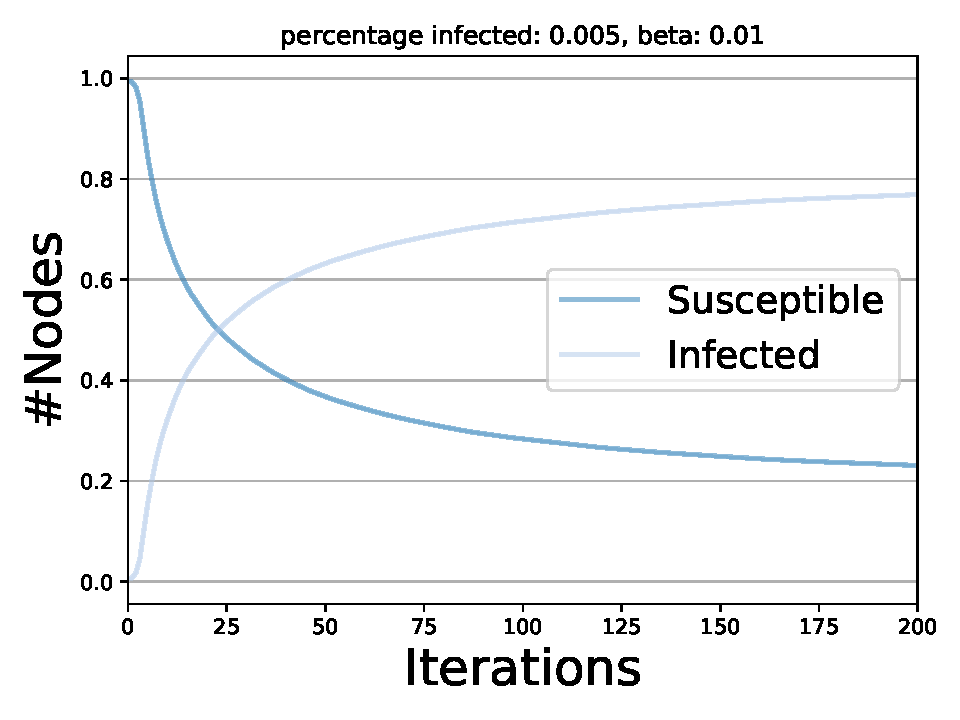
\includegraphics{images/spreading/si/diffusion.pdf}

            }
            \caption{}
            \label{diff_si}
        \end{subfigure}
        \begin{subfigure}{0.45\textwidth}
            \resizebox{\textwidth}{!}{
                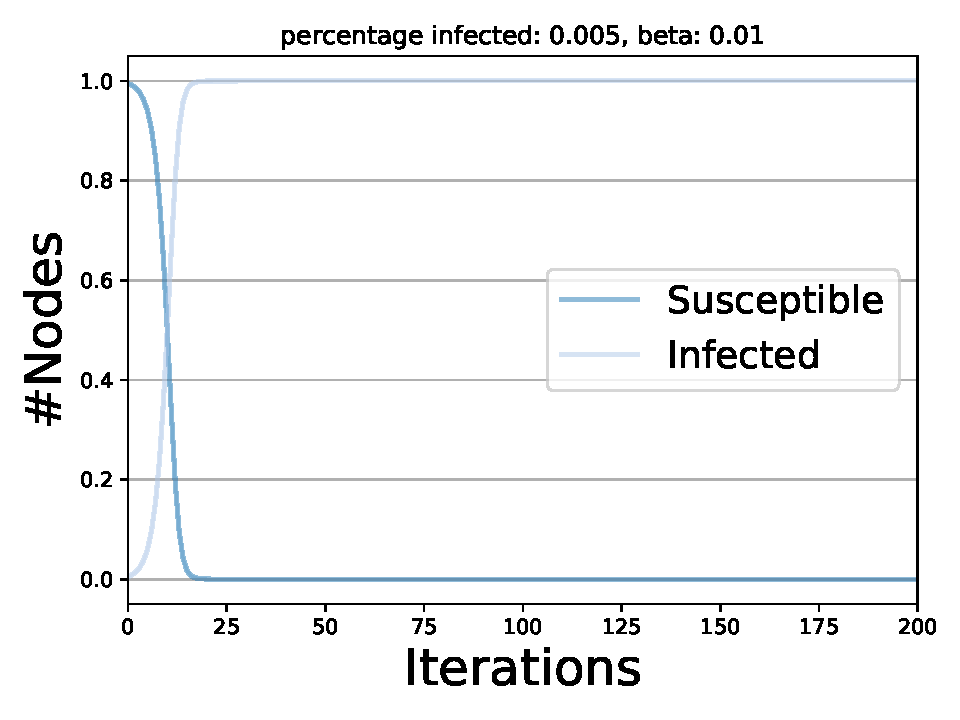
\includegraphics{images/spreading/si/diffusion_er.pdf}
            }
            \caption{}
            \label{diff_si_er}
        \end{subfigure}
        \begin{subfigure}{0.45\textwidth}
            \resizebox{\textwidth}{!}{
                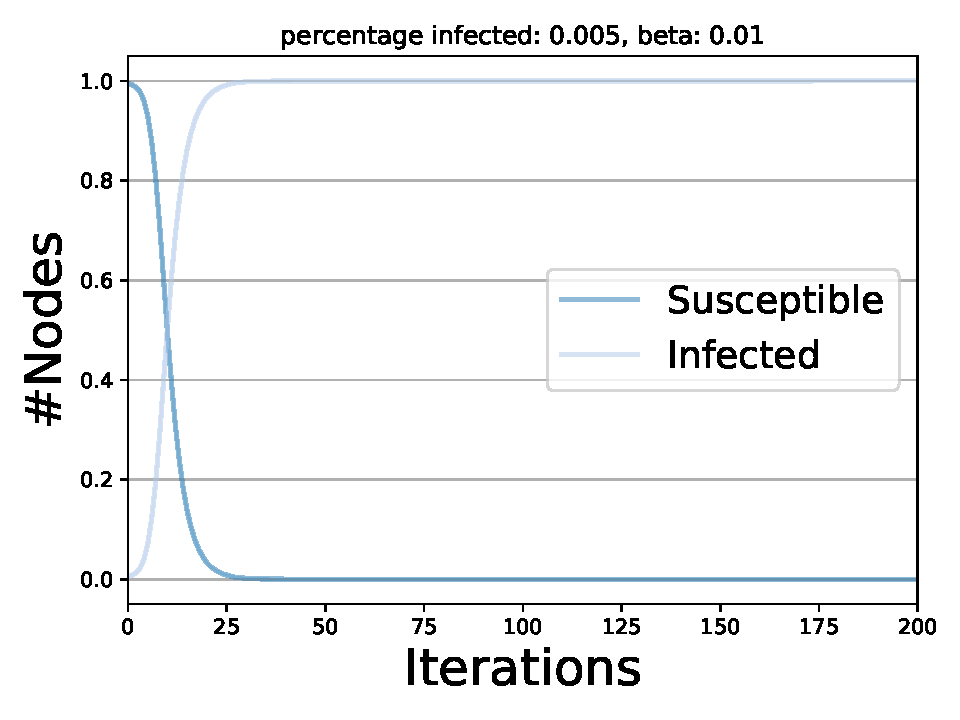
\includegraphics{images/spreading/si/diffusion_ba.pdf}
            }
            \caption{}
            \label{diff_si_ba}
        \end{subfigure}
        \begin{subfigure}{0.45\textwidth}
            \resizebox{\textwidth}{!}{
                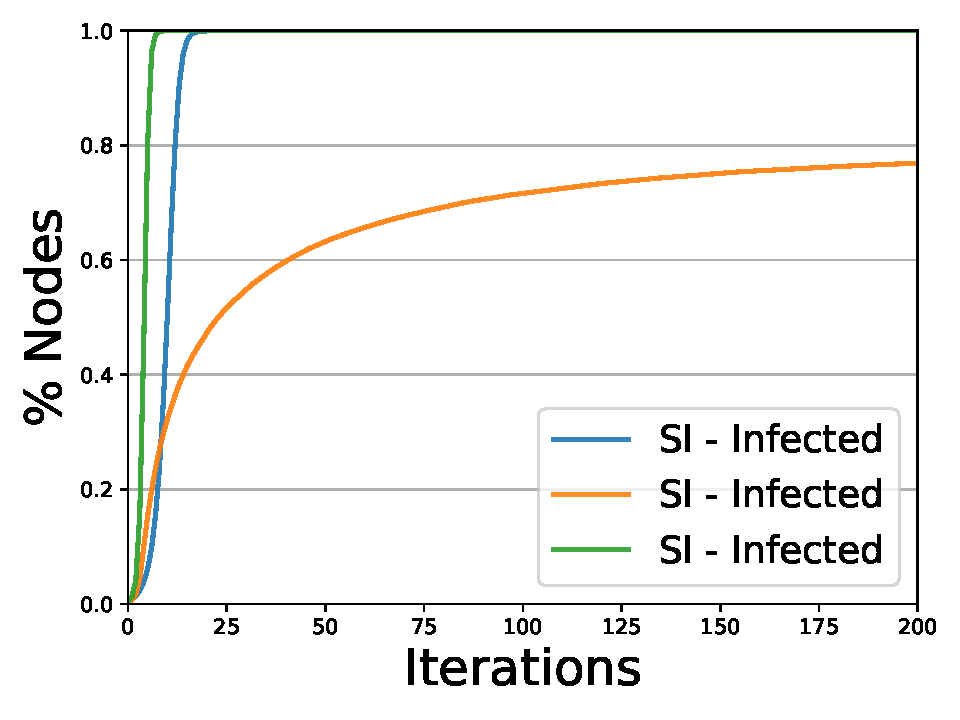
\includegraphics{images/spreading/si/trend_comparison.pdf}
            }
            \caption{}
            \label{diff_si_comparison}
        \end{subfigure}
        \caption{In Figure \ref{diff_si} we can see the diffusion graph for the original network, while in Figure
        \ref{diff_si_er} and in Figure \ref{diff_si_ba} we can see the diffusion graph for the Erdős–Rényi and
        Barabási–Albert networks, respectively. In Figure \ref{diff_si_comparison} we can see a comparison between
        the infection rate of the three networks.}
        \label{diff_si_total}
    \end{figure}
    For the \textbf{Susceptible-Infected} model we've started with a $0.005\%$ of the total population ($3$ nodes)
    of each network being infected, and we've choosed a value of $0.01$ for the infection rate $\beta$. As you can
    see from Figure \ref{diff_si_total}, the original network is the only one that doesn't reach the saturation
    regime, while the other networks reach it within the first $25$ iterations of the model. This is due to the fact
    that both the Erdős–Rényi and the Barabási–Albert network are extremely connected, hence it is more easy for the
    infection to spread among the nodes.

% section si_model (end)

\section{SIS model} % (fold)
\label{sec:sis_model}
    \begin{figure}[H]
        \centering
        \begin{subfigure}{0.45\textwidth}
            \resizebox{\textwidth}{!}{
                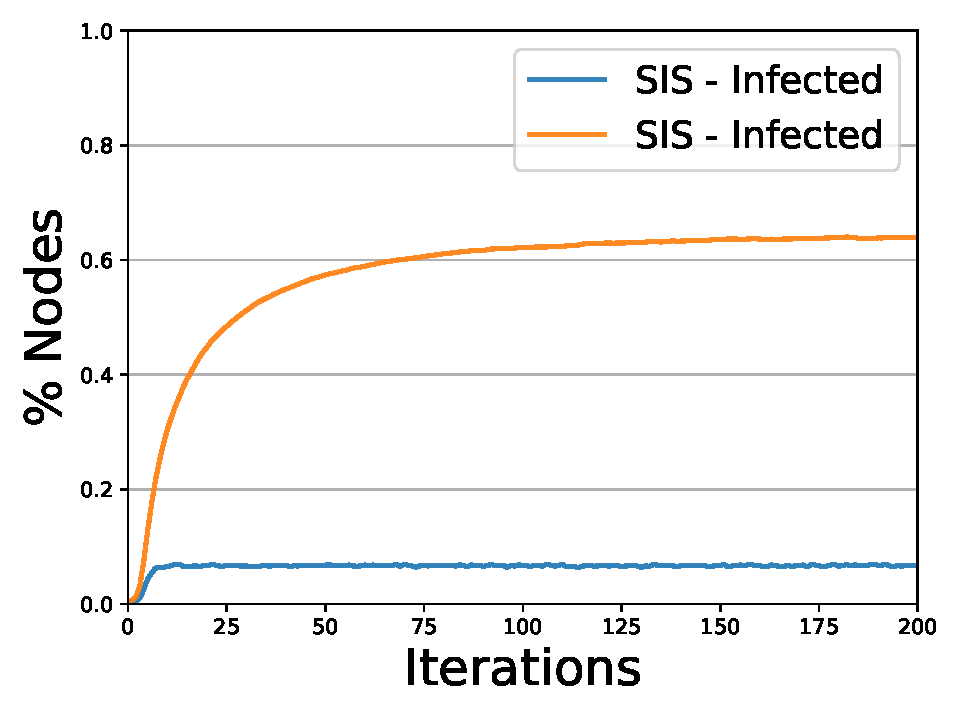
\includegraphics{images/spreading/sis/diffusion_original_comparison.pdf}
            }
            \caption{}
            \label{diff_sis}
        \end{subfigure}
        \begin{subfigure}{0.45\textwidth}
            \resizebox{\textwidth}{!}{
                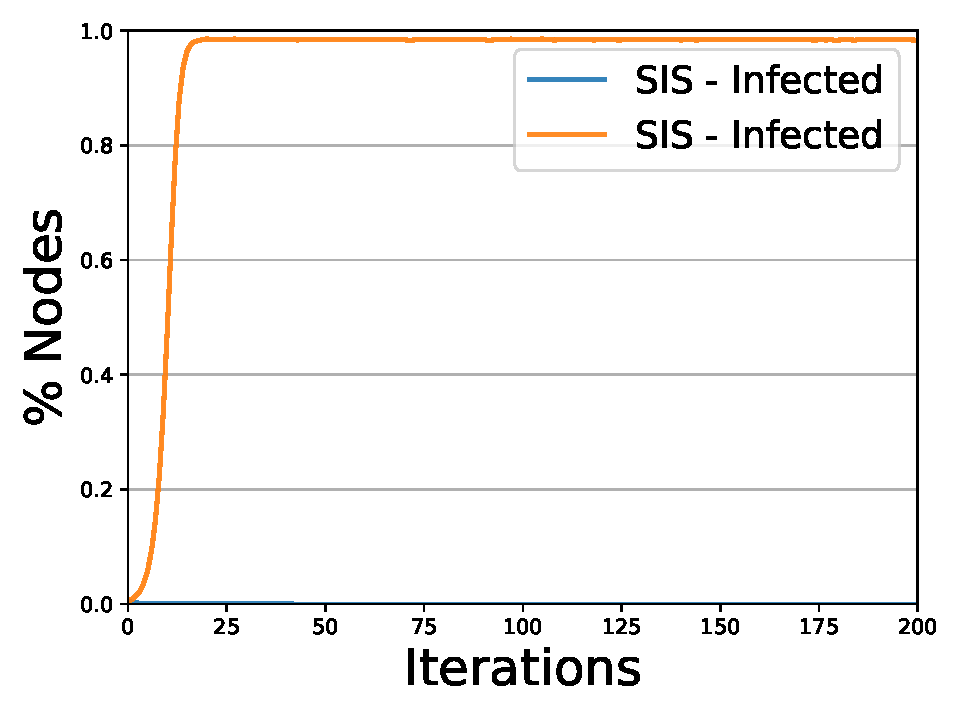
\includegraphics{images/spreading/sis/diffusion_er_comparison.pdf}
            }
            \caption{}
            \label{diff_sis_er}
        \end{subfigure}
        \begin{subfigure}{0.45\textwidth}
            \resizebox{\textwidth}{!}{
                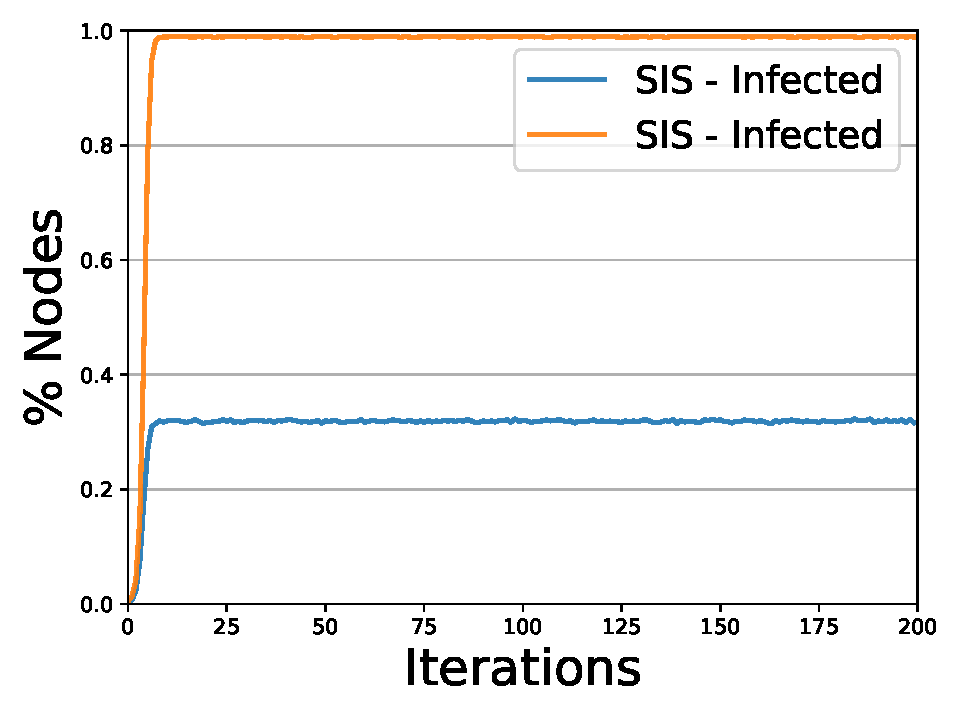
\includegraphics{images/spreading/sis/diffusion_ba_comparison.pdf}
            }
            \caption{}
            \label{diff_sis_ba}
        \end{subfigure}
        \caption{In Figure \ref{diff_sis} we can see the comparison between the endemic state, in orange, and the
        disease free state, in blue, for the original network. The same comparison can be observed for the
        Erdős–Rényi and the Barabási–Albert network, respectively, in Figure \ref{diff_sis_er} and
        \ref{diff_sis_ba}}
        \label{diff_sis_total}
    \end{figure}
    For the \textbf{Susceptible-Infected-Susceptible} model, thanks to the introduction of the recovery rate $\mu$,
    we can model two possible outcomes for the epidemic: the \textbf{endemic state}, characterized by a low recovery
    rate and by the fraction of infected individuals that follows a logistic curve similar to the one observed for
    the SI model, for which $\mu < \beta\langle k \rangle$, and the \textbf{disease free} state, characterized by a
    sufficiently high recovery rate, for which $\mu > \beta\langle k \rangle$. A comparison between this two states
    is represented for every network in Figure \ref{diff_sis_total}.

% section sis_model (end)

\section{SIR model} % (fold){}
\label{sec:sir_model}
    The key characteristic of the \textbf{Susceptible-Infected-Recovered} model consist in introducing the
    probability $\gamma$ for the individuals to recover from the disease and hence to be "removed" from the
    population instead of returning to the susceptible state. We have choosen to test this model either for the case
    in which $\gamma$ is smaller than $\beta$ and the other way around. The graphs representing this different
    situations for all the three networks are visible in Figure \ref{diff_sir_total}.
    \begin{figure}
        \begin{subfigure}{0.33\textwidth}
            \resizebox{\textwidth}{!}{
                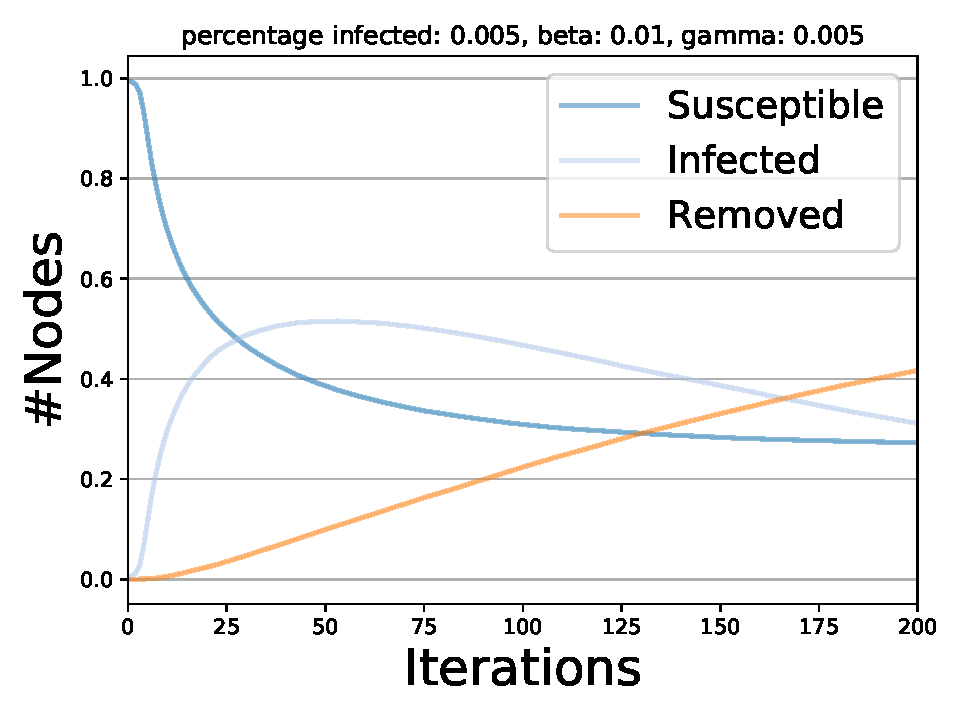
\includegraphics{images/spreading/sir/diffusion_smaller.pdf}
            }
            \caption{}
            \label{diff_sir_smaller}
        \end{subfigure}
        \begin{subfigure}{0.33\textwidth}
            \resizebox{\textwidth}{!}{
                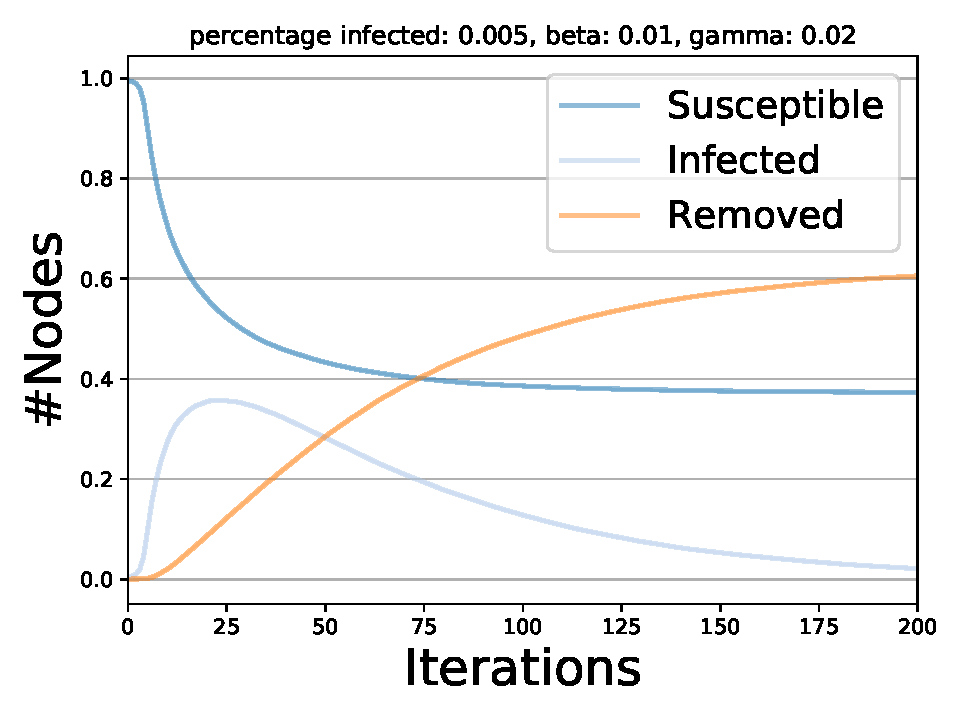
\includegraphics{images/spreading/sir/diffusion_greater.pdf}
            }
            \caption{}
            \label{diff_sir_greater}
        \end{subfigure}
        \begin{subfigure}{0.33\textwidth}
            \resizebox{\textwidth}{!}{
                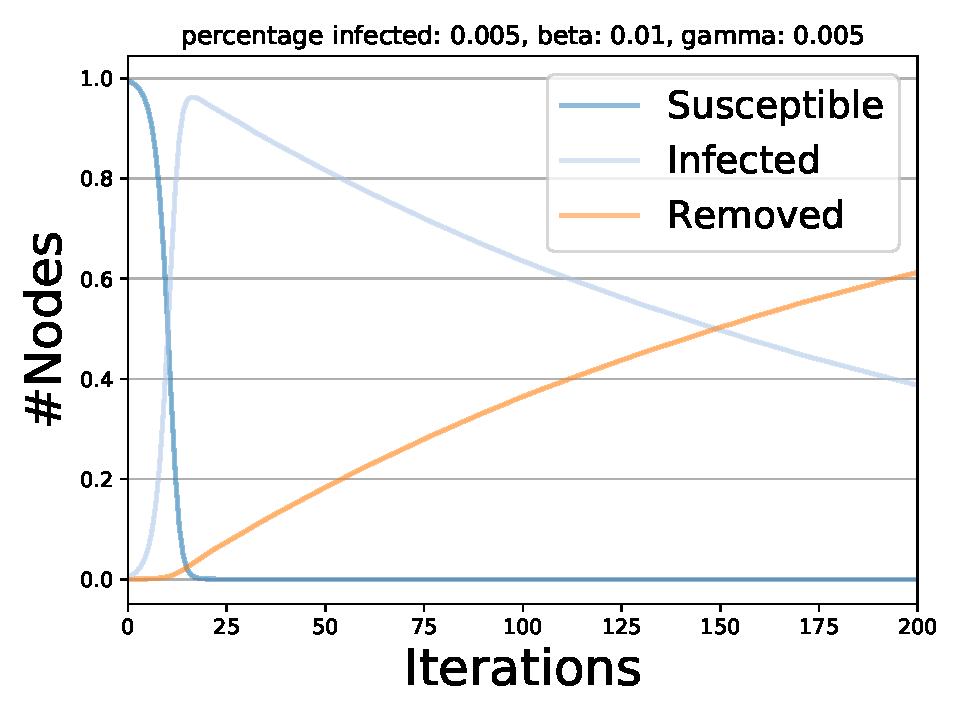
\includegraphics{images/spreading/sir/diffusion_er_smaller.pdf}
            }
            \caption{}
            \label{diff_sir_er_smaller}
        \end{subfigure}
        \begin{subfigure}{0.33\textwidth}
            \resizebox{\textwidth}{!}{
                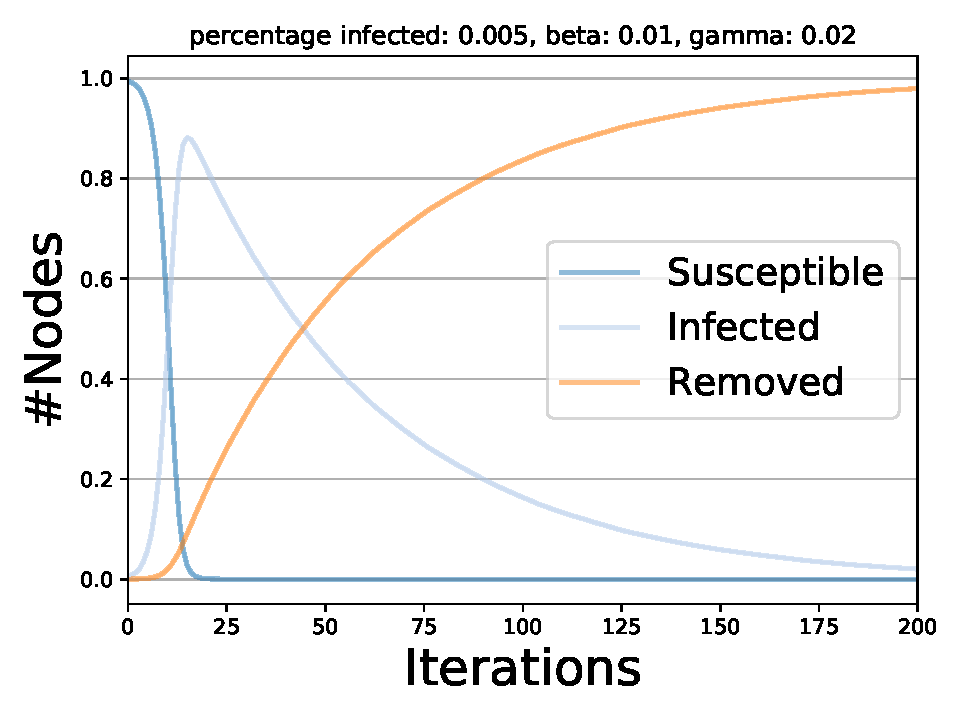
\includegraphics{images/spreading/sir/diffusion_er_greater.pdf}
            }
            \caption{}
            \label{diff_sir_er_greater}
        \end{subfigure}
        \begin{subfigure}{0.33\textwidth}
            \resizebox{\textwidth}{!}{
                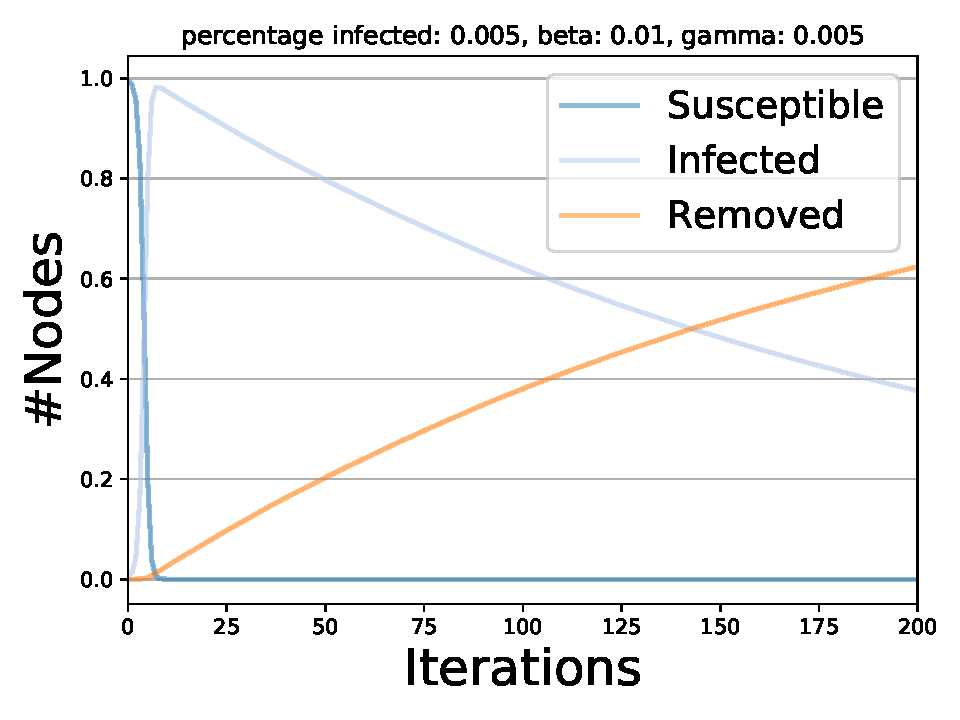
\includegraphics{images/spreading/sir/diffusion_ba_smaller.pdf}
            }
            \caption{}
            \label{diff_sir_ba_smaller}
        \end{subfigure}
        \begin{subfigure}{0.33\textwidth}
            \resizebox{\textwidth}{!}{
                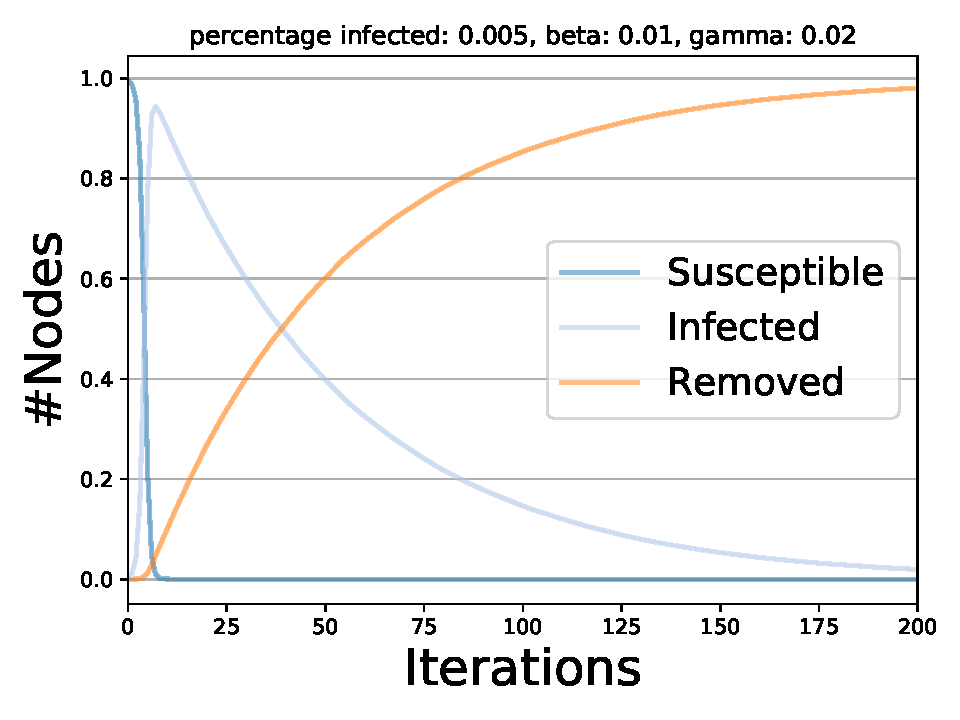
\includegraphics{images/spreading/sir/diffusion_ba_greater.pdf}
            }
            \caption{}
            \label{diff_sir_ba_greater}
        \end{subfigure}
        \caption{In Figure \ref{diff_sir_smaller} and \ref{diff_sir_greater} we can see the representation of the
        diffusion on the original network both for the case in which $\gamma$ is smaller than $\beta$ and the other
        way around. The same kind of representation is plotted for the Erdős–Rényi network in Figure
        \ref{diff_sir_er_smaller} and \ref{diff_sir_er_greater} and for the Barabási–Albert network in Figure
        \ref{diff_sir_ba_smaller} and \ref{diff_sir_ba_greater}.}
        \label{diff_sir_total}
    \end{figure}

% section sir_model (end)

\section{Threshold model} % (fold)
\label{sec:threshold_model}
    Finally we describe the application of the \textbf{Threshold model} both on the original network and the
    synthetic ones. In order to test this model we've choosen to apply a threshold $\tau$ eguals to $0.10$, the
    diffusion of the infection for this model is represented in Figure \ref{diff_thr_total}. As we can see, for the
    original network we have that almost all the nodes become infected within the first $20$ model's iterations,
    due to the fact that the value choosen for the threshold results to be sufficient for the spreading of the
    infection. If we change the threshold's value, this time using $0.20$, we can observe that the
    original network become immune to the infection, thanks to its internal structure. We can observe
    the same immunity in the Erdős–Rényi and Barabási–Albert network for the original threshold's value.
    \begin{figure}[H]
        \centering
        \begin{subfigure}{0.33\textwidth}
            \resizebox{\textwidth}{!}{
                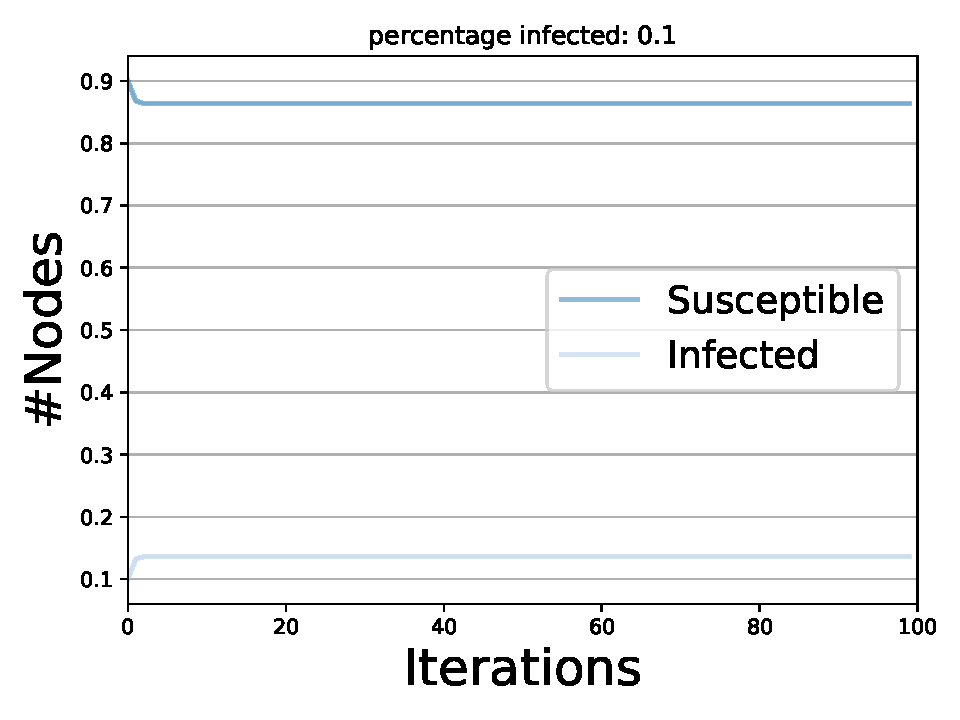
\includegraphics{images/spreading/threshold/diffusion.pdf}
            }
            \caption{}
            \label{diff_thr}
        \end{subfigure}
        \begin{subfigure}{0.33\textwidth}
            \resizebox{\textwidth}{!}{
                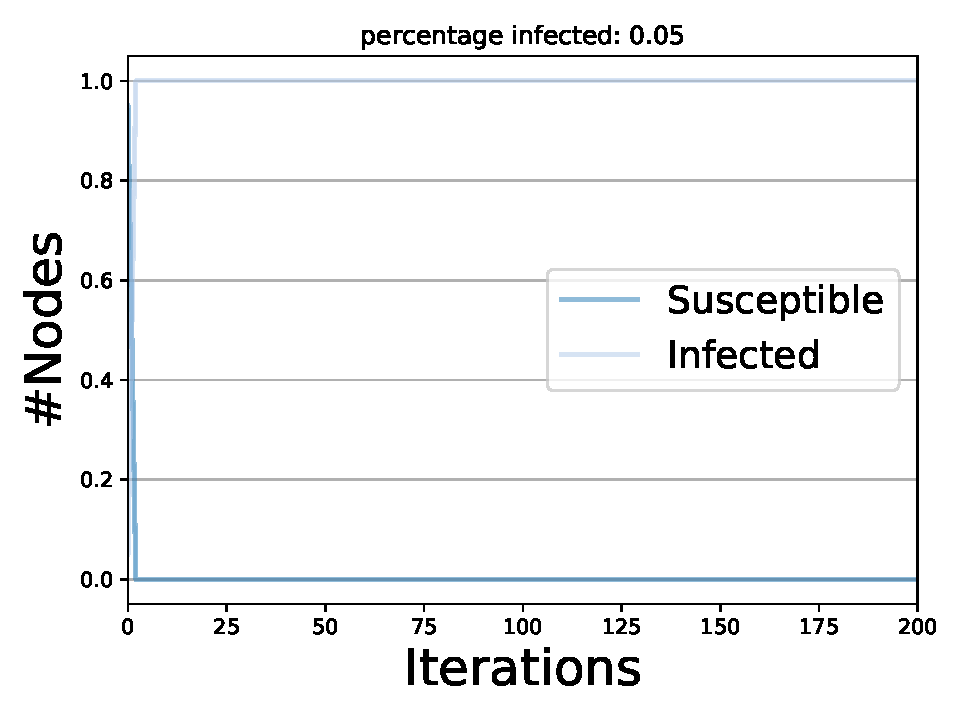
\includegraphics{images/spreading/threshold/diffusion_er.pdf}
            }
            \caption{}
            \label{diff_thr_er}
        \end{subfigure}
        \begin{subfigure}{0.33\textwidth}
            \resizebox{\textwidth}{!}{
                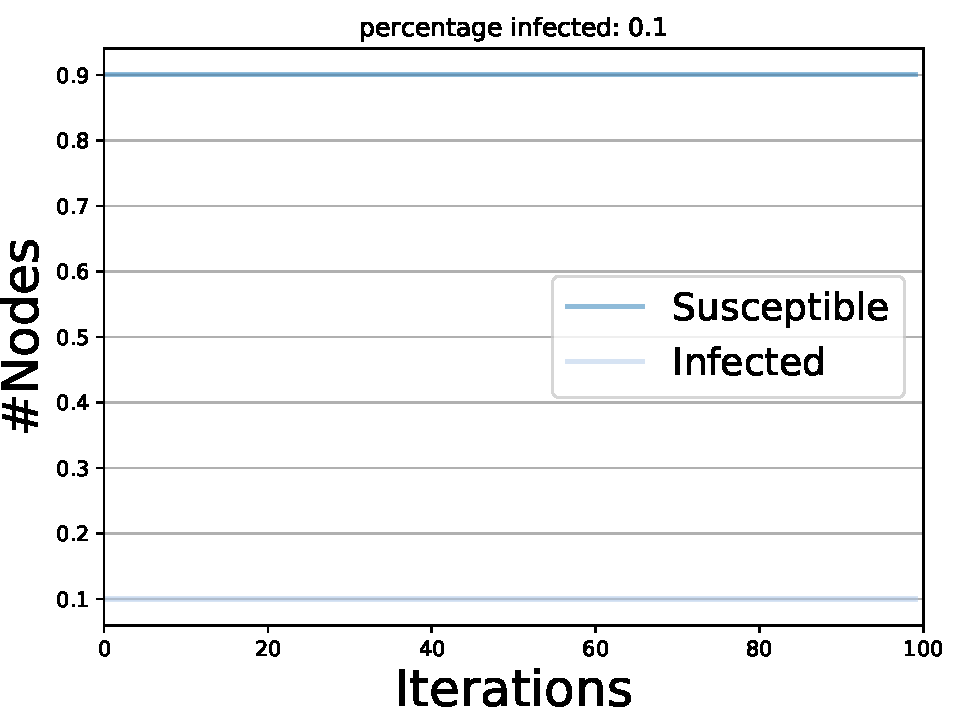
\includegraphics{images/spreading/threshold/diffusion_ba.pdf}
            }
            \caption{}
            \label{diff_thr_ba}
        \end{subfigure}
        \begin{subfigure}{0.33\textwidth}
            \resizebox{\textwidth}{!}{
                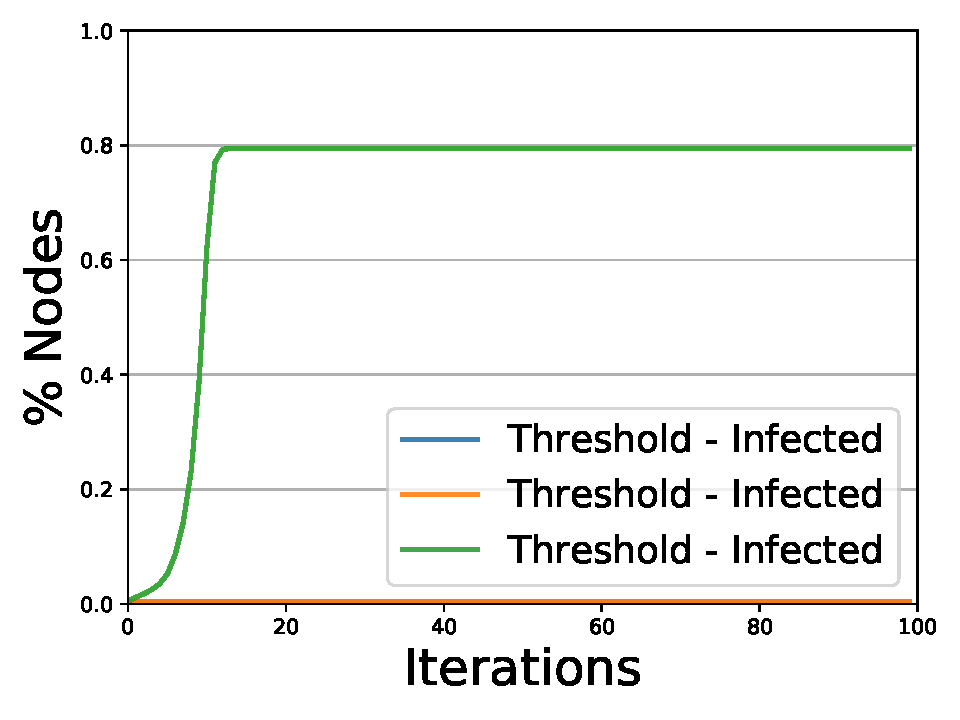
\includegraphics{images/spreading/threshold/trend_comparison.pdf}
            }
            \caption{}
            \label{diff_thr_comparison}
        \end{subfigure}
        \caption{In Figure \ref{diff_thr} is represented the diffusion of the infection for the original network,
        while in Figure \ref{diff_thr_er} and \ref{diff_thr_ba} are represented the cases for the Erdős–Rényi and
        the Barabási–Albert network, respectively. A comparison between the three networks is represented in Figure
        \ref{diff_thr_comparison}.}
        \label{diff_thr_total}
    \end{figure}

% section threshold_model (end)

% chapter spreading (end)


    \chapter{Summary}


\printbibliography[title={References}]


\end{document}
